\paragraph{Sơ đồ tuần tự luồng Hủy liên kết và thiết lập lại thiết bị MFA}

Luồng nghiệp vụ này mô tả
chi tiết quy trình người dùng hủy liên kết thiết bị MFA hiện tại trong trang cá nhân, sau đó thiết lập lại thiết bị xác thực mới thông qua trang \texttt{/auth/mfa} và Supabase Auth Service.

\begin{figure}[H]
\centering
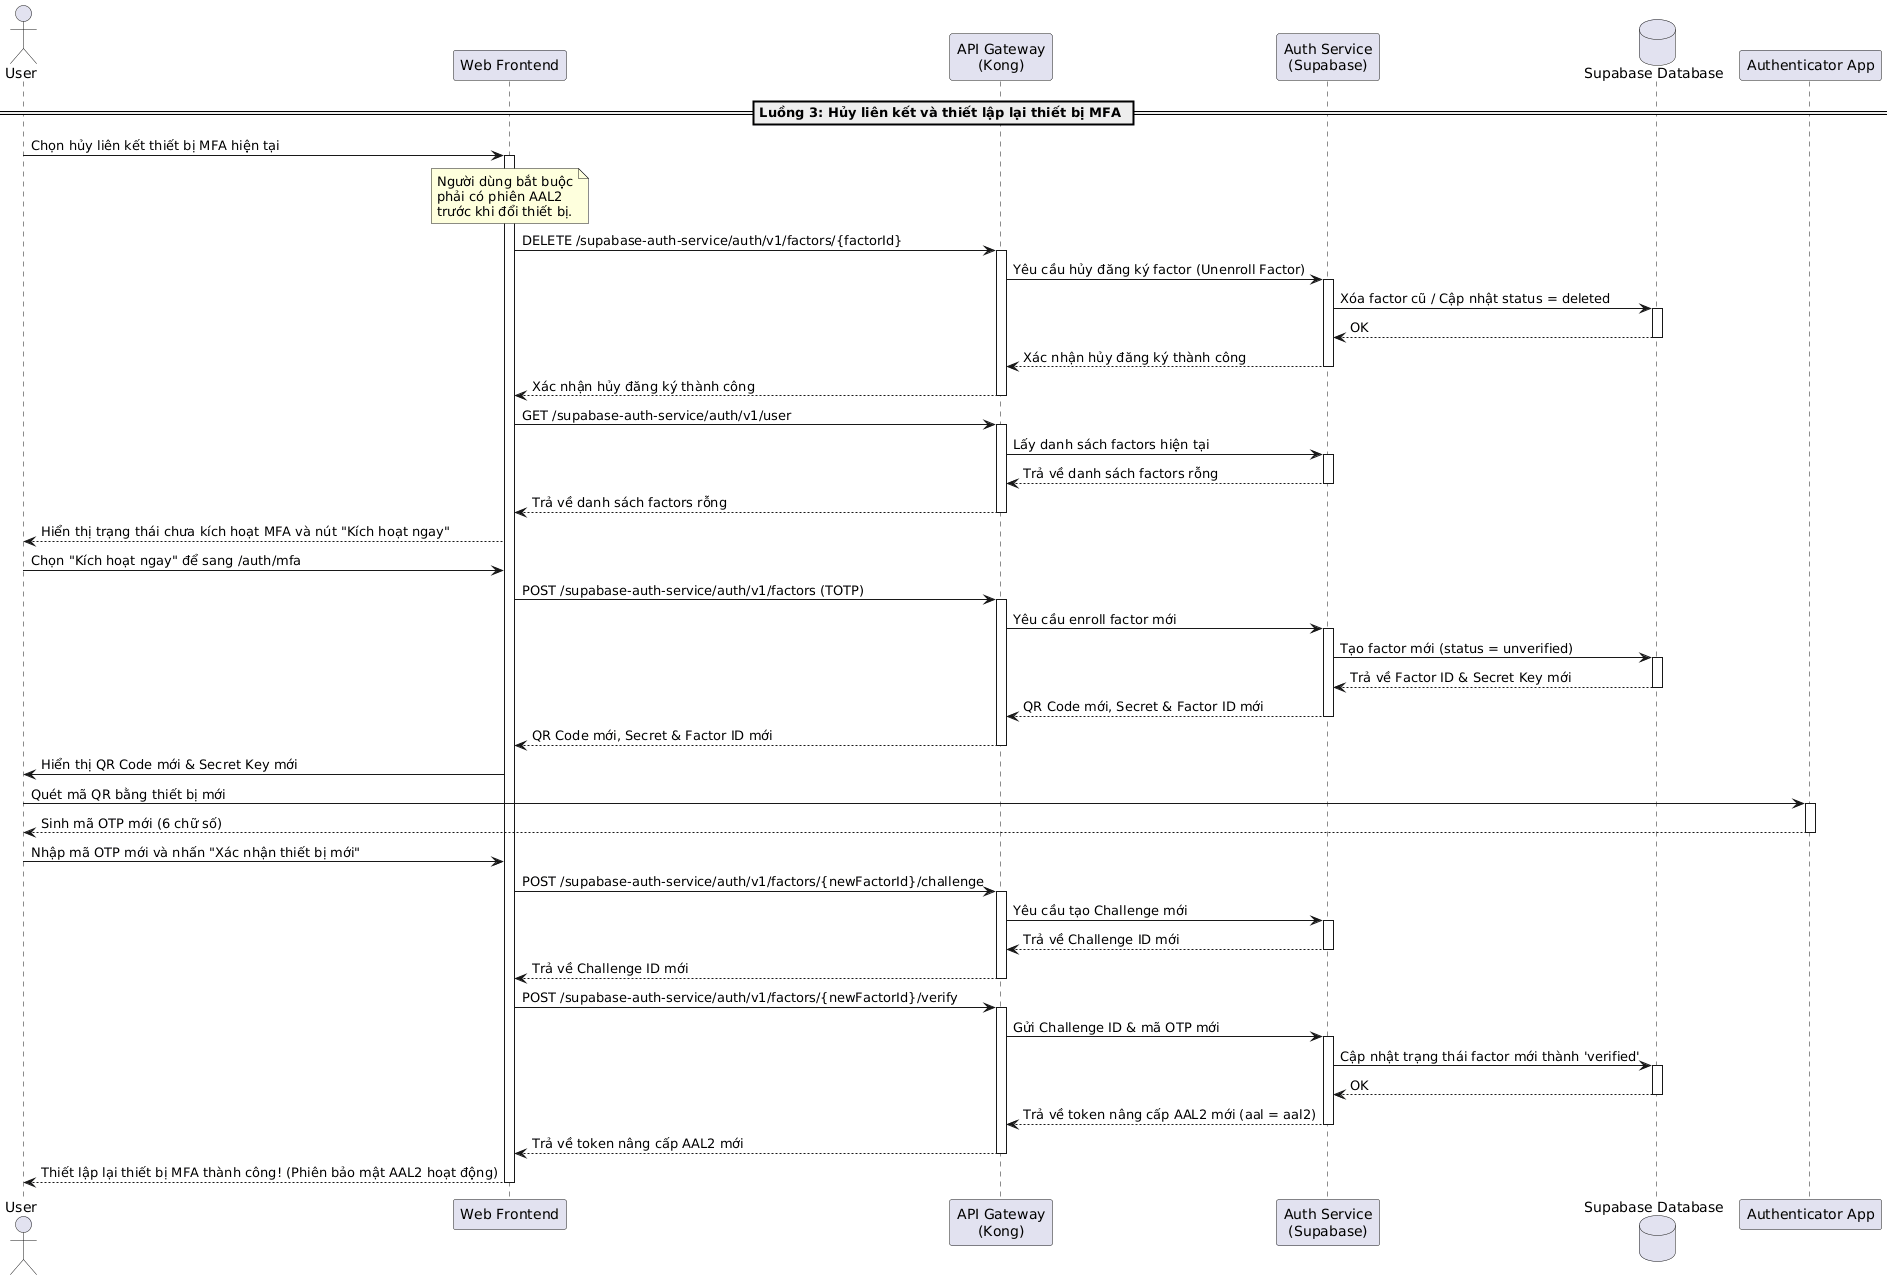
\includegraphics[scale = 0.22]{contents/Sequence/UML-Sequence-UserMfaResetDevice.png}
\caption{Sơ đồ tuần tự luồng Hủy liên kết và thiết lập lại thiết bị MFA}
\end{figure}

\subparagraph{Các thành phần tham gia}

\begin{table}[H]
\centering
\renewcommand{\arraystretch}{1.3}

\begin{tabular}{|l|l|p{5cm}|}
\hline
\textbf{Thành phần} & \textbf{Phân loại} & \textbf{Vai trò trong hệ thống} \\ \hline
User & Actor & Người dùng thực hiện thay đổi thiết bị bảo mật. \\ \hline
Web Frontend & Component & Giao diện web Next.js. \\ \hline
API Gateway (Kong) & Component & Cổng API chuyển tiếp các yêu cầu API. \\ \hline
Auth Service (Supabase) & Microservice & Dịch vụ thực hiện hủy đăng ký thiết bị cũ và xử lý thiết bị mới. \\ \hline
Authenticator App & External Service & Ứng dụng di động mới của người dùng thực hiện quét QR và sinh TOTP xác thực. \\ \hline
\end{tabular}
\caption{Các thành phần tham gia luồng Hủy liên kết và thiết lập lại thiết bị MFA}
\end{table}

\subparagraph{Mô tả tổng quan}

\begin{itemize}
\item \textbf{Yêu cầu hủy thiết bị cũ:} Để thay đổi thiết bị xác thực hai lớp, người dùng yêu cầu hủy liên kết với thiết bị cũ trong trang quản lý tài khoản cá nhân trên giao diện. Yêu cầu này chỉ được chấp nhận khi phiên đăng nhập hiện tại đã đạt mức bảo mật cao nhất.
\item \textbf{Hủy liên kết:} Giao diện gửi yêu cầu hủy liên kết thiết bị qua cổng API tới dịch vụ chứng thực. Dịch vụ chứng thực xóa thiết bị xác thực cũ khỏi hệ thống và phản hồi thành công về giao diện.
\item \textbf{Bắt đầu thiết lập thiết bị mới:} Giao diện cập nhật lại trạng thái tài khoản sang chưa kích hoạt xác thực hai lớp. Khi người dùng chọn kích hoạt lại, giao diện điều hướng sang trang thiết lập xác thực hai lớp và gửi yêu cầu đăng ký để nhận mã phản hồi nhanh và khóa bảo mật mới cho thiết bị mới.
\item \textbf{Xác thực thiết bị mới:} Người dùng quét mã phản hồi nhanh bằng ứng dụng xác thực mới và nhập mã xác thực mới. Giao diện gửi các yêu cầu xác minh để hoàn tất. Khi thành công, dịch vụ chứng thực kích hoạt thiết bị mới và cấp lại mã đăng nhập ở mức bảo mật cao nhất để khôi phục quyền truy cập.
\end{itemize}
